\documentclass[a4paper]{article}
\usepackage{graphicx}
\graphicspath{ {./img/} }

\begin{document}
\title{Computer Architecture Lab 3 Report}
\author{Fabian Wüthrich}
\date{November 2020}
\maketitle

\noindent
The task of this lab is to extend Ramulator to evaluate two memory scheduling
policies: ATLAS and BLISS. Before the actual implementation of the new
policies, the scheduler was refactored using the strategy design pattern to
make the code easier to extend. The refactoring removes many nested
if-statements and moves fields, that were only relevant to certain policies, to
the respective policy class.

\section*{Task 1: Implementing ATLAS}

For implementing ATLAS, we need to track for each thread the attained service
(AS) in the current quantum and the overall AS (TotalAS) up to the current quantum.
Ramulator executes only one thread per core, so \verb|coreid| is used
to identify a thread.

Each memory controller (see \verb|Controller.h|) tracks the AS of
a thread during a quantum in the vector \verb|attained_service|. When a request
is issued, the corresponding vector entry is incremented. The counter is
enclosed in a if-statement so the counter is only incremented on the first
command of a request (see line 417).

ATLAS requires a meta-controller to coordinate multiple memory controllers. The
meta-controller is implemented in the \verb|Memory| class because the class
holds references to all memory controllers. At the end of a quantum, the
meta-controller fetches and accumulates the AS values for each thread (see
line 295-302 in \verb|Memory.h|). Then, the meta-controller recalculates the
TotalAS for each thread and passes the new value to all memory-controllers
(see line 304-313).

The actual policy is implemented in \verb|Scheduler.h| by overriding the
\verb|compare()| function. The scheduler compares the arrival time of a request
to the clock count of the memory controller to figure out if the request has
been outstanding for more than T cycles (see line 229-233) . If both requests
are below the threshold T, the scheduler queries the TotalAS value for each
request from the memory controller and picks the request with the lowest value
(see line 235-241).  If both AS values are the same, the scheduler prioritizes
row hits and then oldest requests first.

\section*{Task 2: Implementing BLISS}

BLISS requires even less machinery than ATLAS and is implemented in
\verb|Controller.h|. The vector \verb|blacklisted| keeps track of the
blacklisted threads. Two variables (\verb|last_request_coreid| and
\verb|request_served_counter|) are used to identify malicious threads.

Similar to ATLAS the \verb|compare()| function is used to pick the best request.
The scheduler returns the request whose thread is not blacklisted or defaults to
row hits/oldest first if a decision based on the blacklist is not possible.

\section*{Task 3: Evaluation}

%TODO Say that BLISS got faster when I moved it into first_command if

\begin{figure}
    \centering
    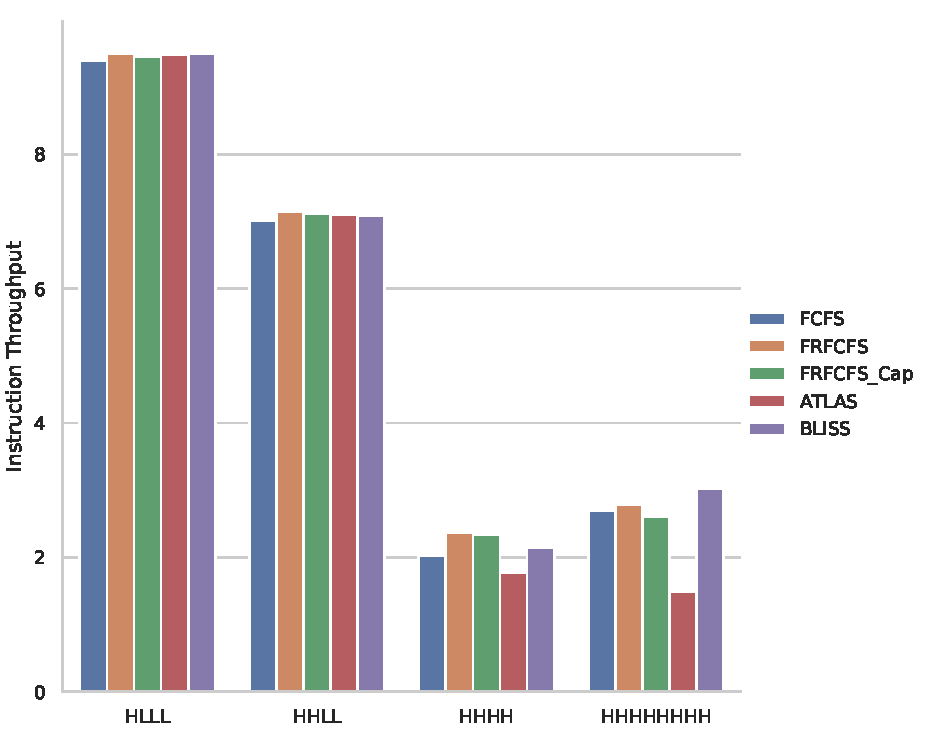
\includegraphics[width=\textwidth]{inst_throughput}
    \caption{Instruction Throughput}
    \label{fig:inst-througput}
\end{figure}

\begin{figure}
    \centering
    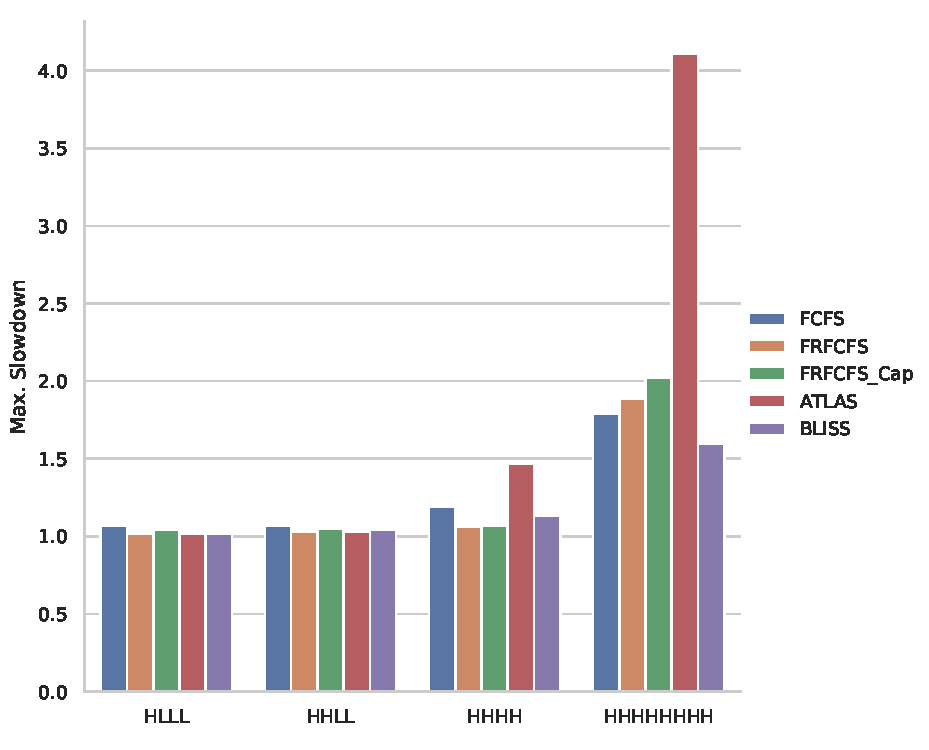
\includegraphics[width=\textwidth]{max_slowdown}
    \caption{Max. Slowdown}
    \label{fig:max-slowdown}
\end{figure}


\end{document}
